

%%%%%%%%%%%%%%%%%%%%%%%%%%%%%%%%%%%%%%%%%%%%%%%%%%%%%%%%%%%%%%%%%%%%%%%%%%%%%%%%%%%%%%%%%%%%%%%%%%%%%%%%%


%
\newpage
\section{Предлагаемая схема информационных потоков в БП}

\subsection{Процессы ''Подготовка производства'', ''Учет технологической оснастки''}
%%
\begin{figure}
\begin{center}
  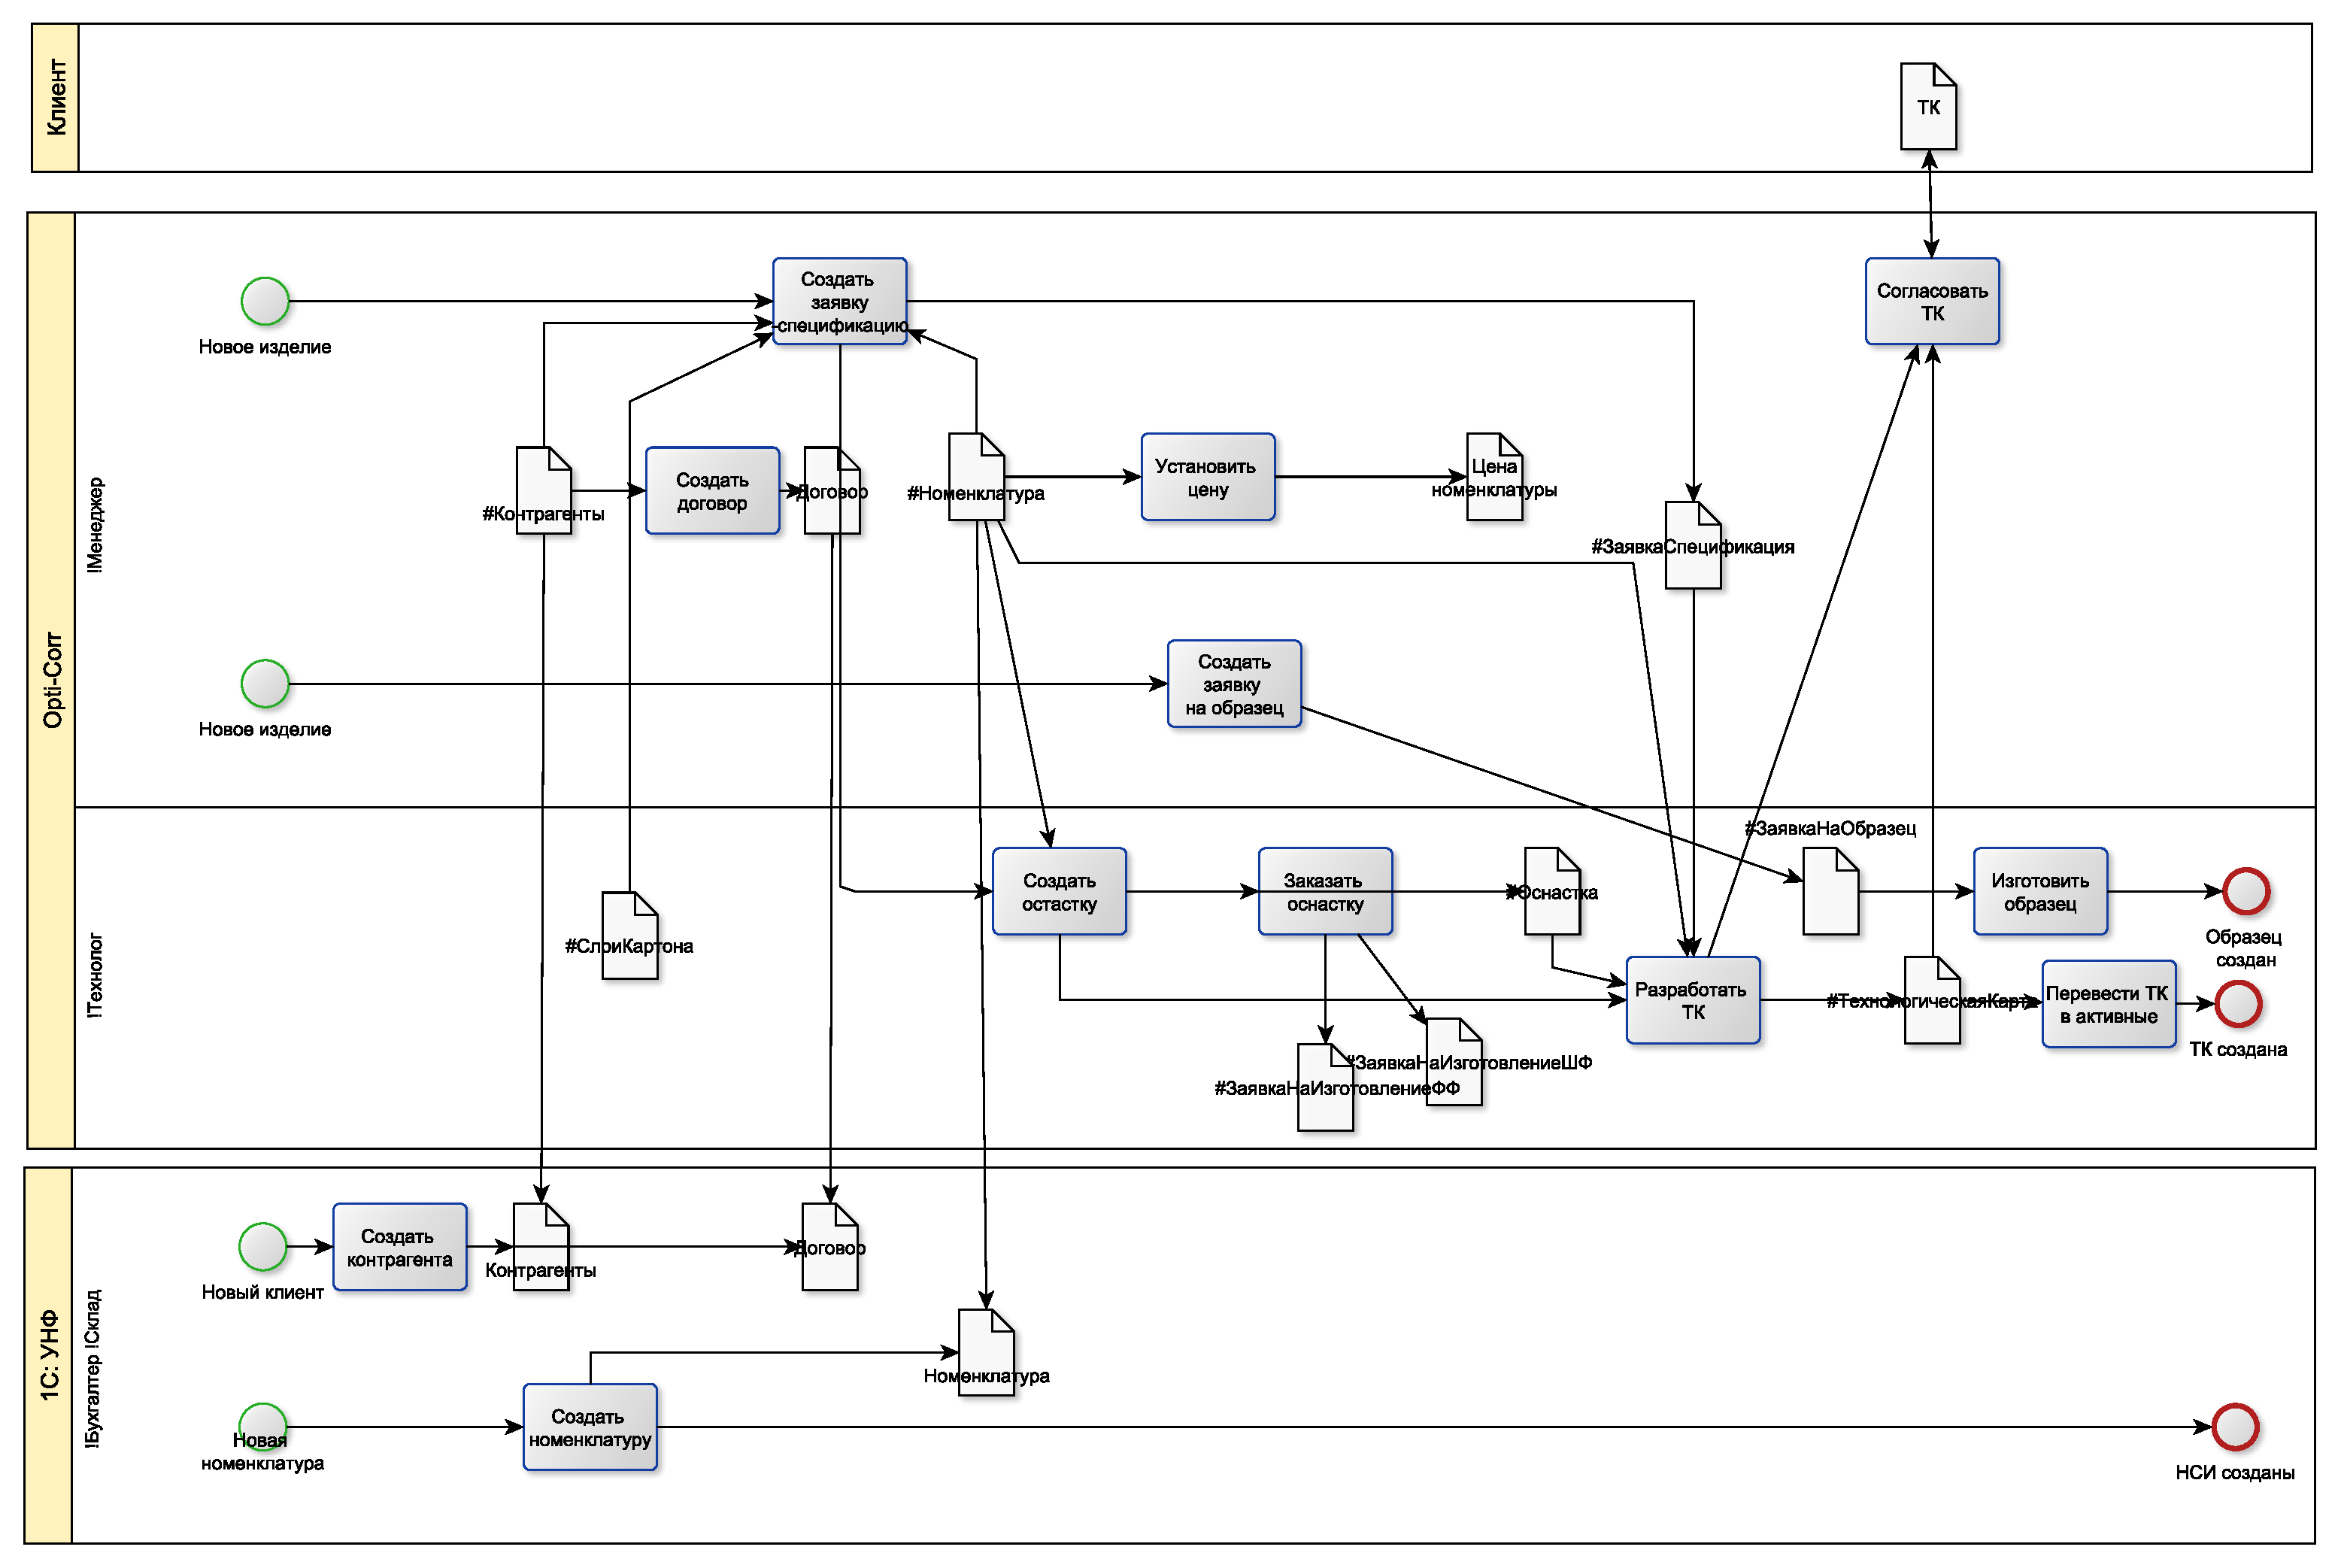
\includegraphics[angle=90, height=0.9\textheight, keepaspectratio]{Pics/1_NewGoods.pdf}
\end{center}
  \caption{Процессы ''Подготовка производства'', ''Учет технологической оснастки''}
  \label{pic:Schema_1}
\end{figure}
\clearpage

При появлении нового контрагента менеджер будет создавать в справочнике ''Контрагенты'' новый элемент справочника в системе Opti-Corrugated (Опти-Софт) для покупателей и в системе 1С:УНФ для других контрагентов (см. рис. \ref{pic:Schema_1}).


При автоматическом обмене 1С:УНФ выгрузит новый элемент ''Контрагенты'' в систему  Опти-Софт (СИСТЕМА). При обмене справочники ''Контрагенты'' будут синхронизированы. 

Менеджер при появлении требований от заказчика рассчитывает цену продажи изделия в таблице MS EXCEL. После согласования цены при необходимости менеджер создает автоматически номенклатуру нового изделия в справочнике ''Номенклатура'' в СИСТЕМЕ. 

При автоматическом обмене система 1С:УНФ выгрузит новый элемент ''Номенклатура'' в систему Опти-Софт и загрузит новые обратно. При обмене справочники ''Номенклатура'' будут синхронизированы. 

% На основании выполненного расчета цены менеджер формирует печатную форму коммерческого предложения и высылает клиенту. %Есть возможность выслать предложение прямо из СИСТЕМЫ.
% Менеджер будет формировать печатную форму договора и спецификации цены из системы 1С:УНФ. 

После согласования цены менеджер создает в СИСТЕМЕ документ ''Заявка-спецификация'' -- распоряжение технологу по разработке оснастки и технологической карты. 

Отдел главного технолога создает технологическую карту в СИСТЕМЕ, которую менеджер должен согласовать в печатном виде с заказчиком. 



\subsection{Процессы ''Управление продажами''}
%%
\begin{figure}
\begin{center}
  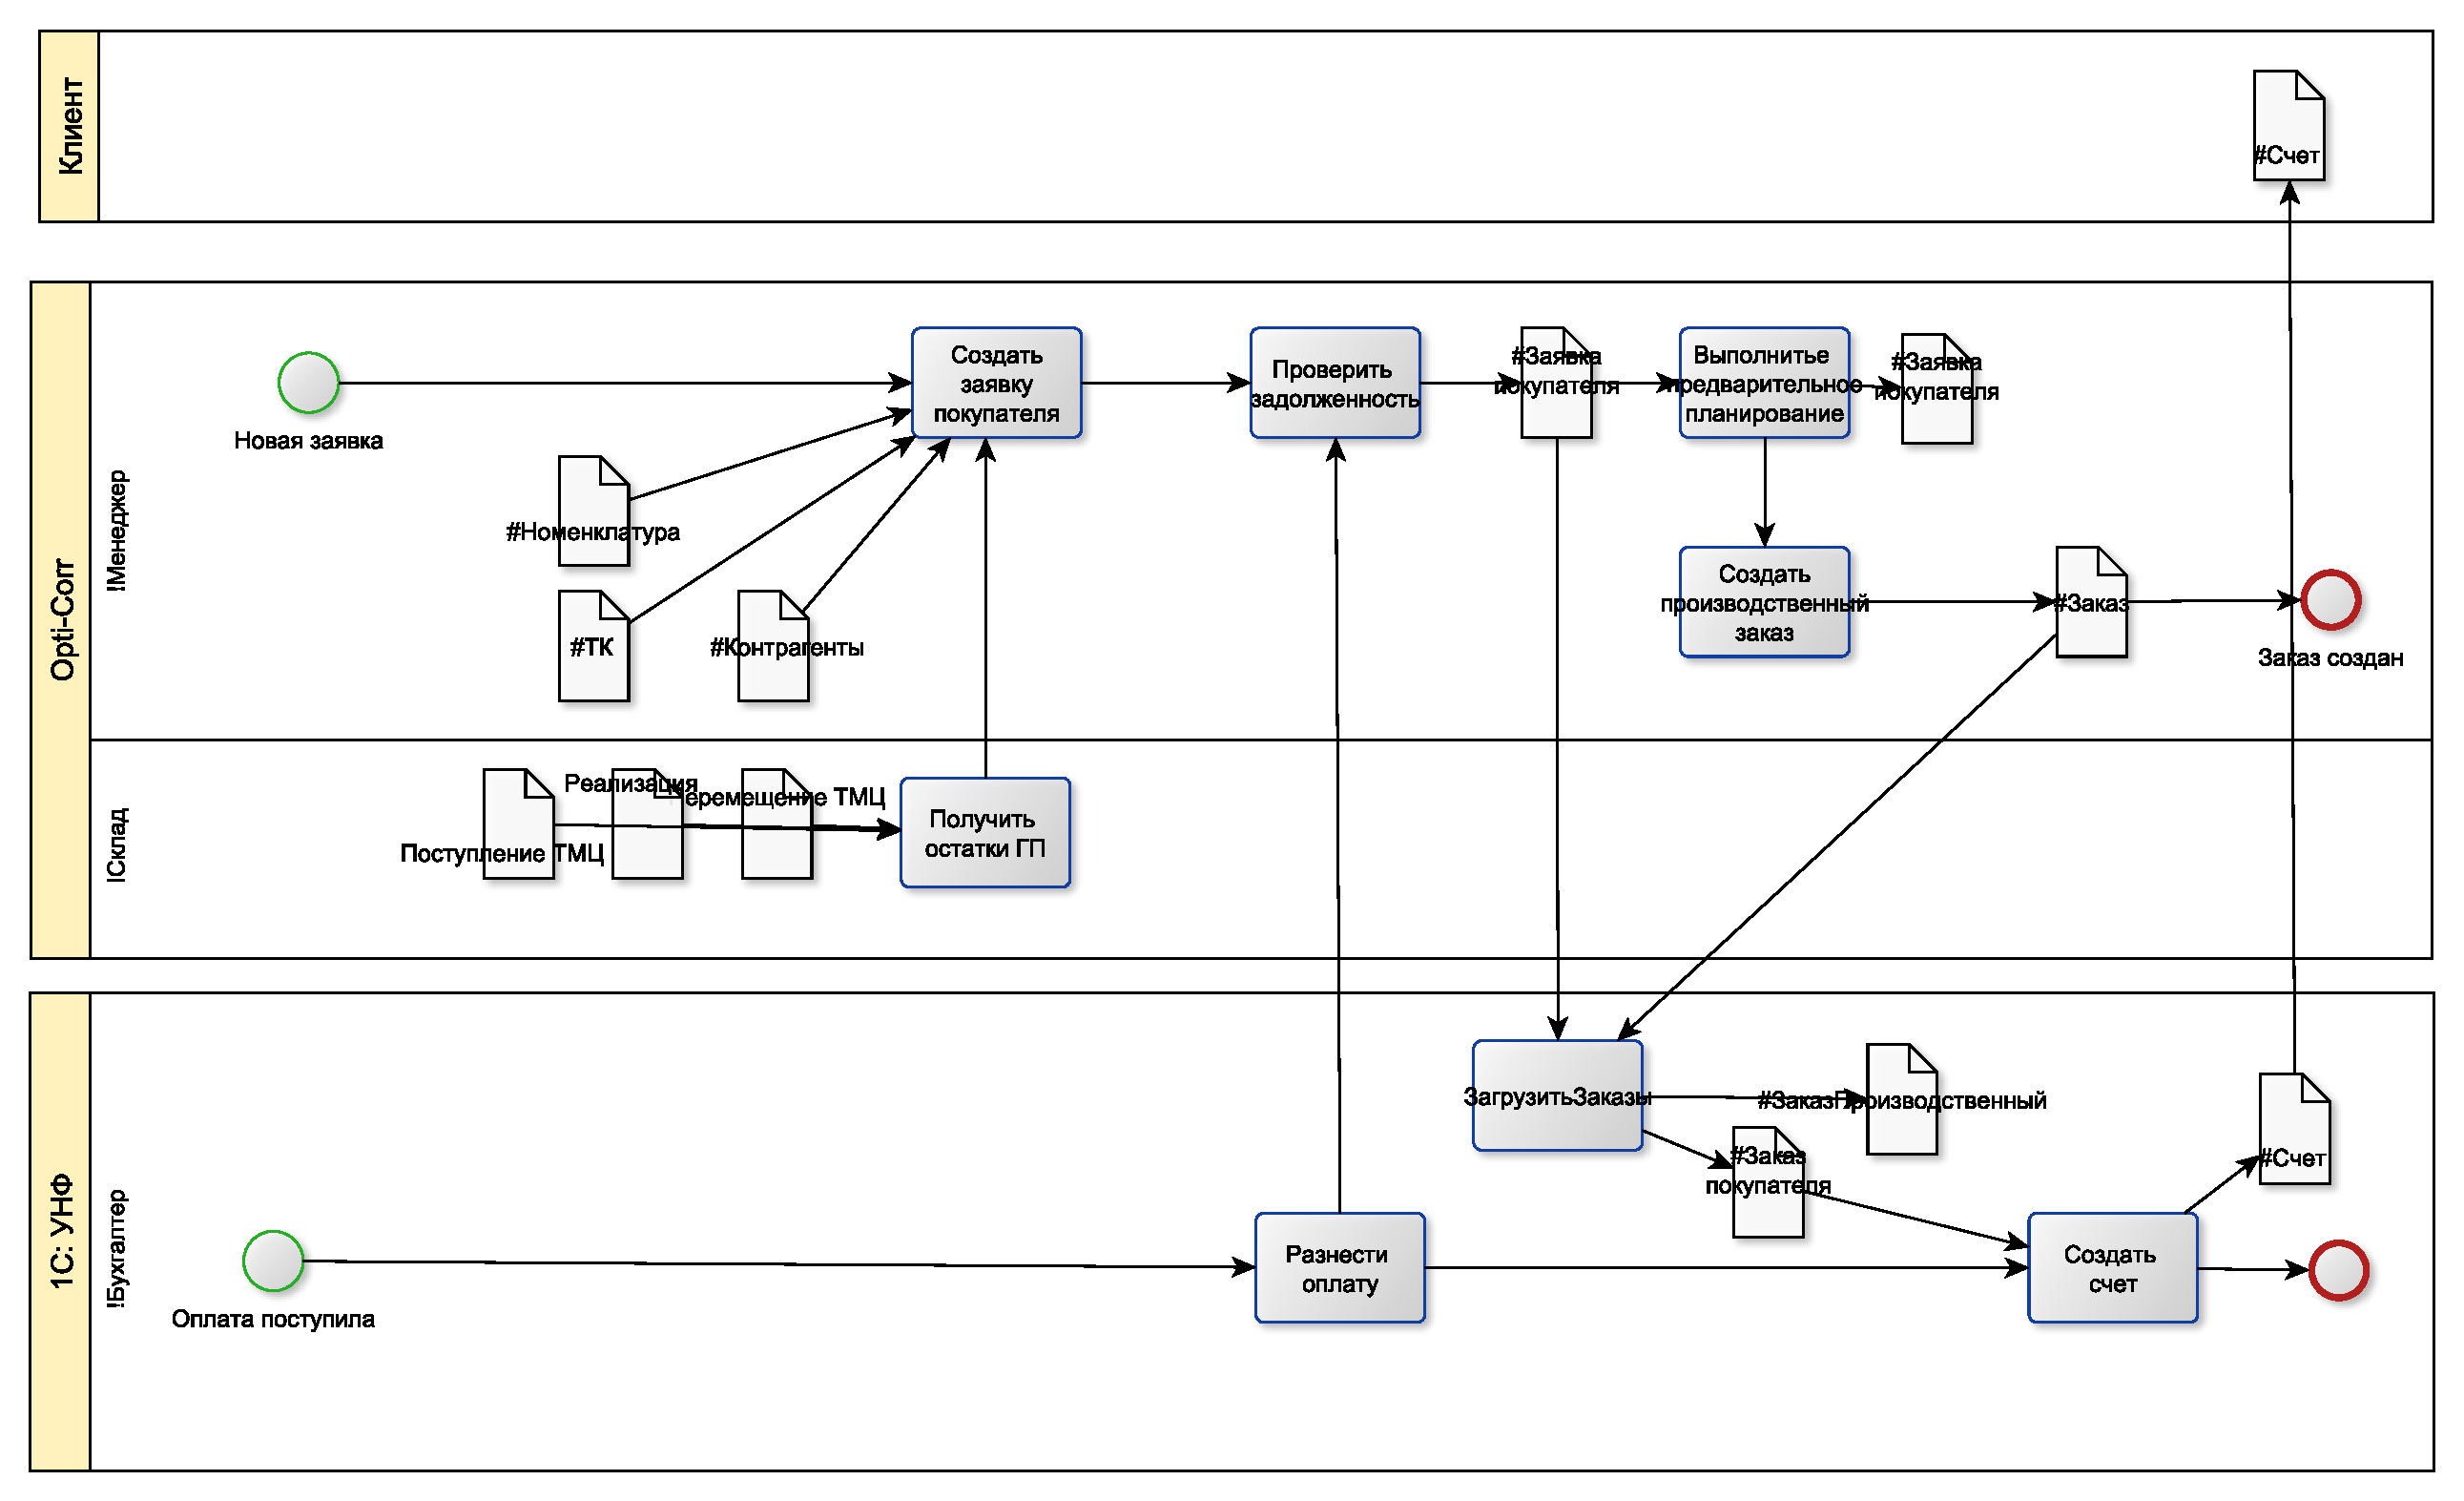
\includegraphics[angle=90, height=0.9\textheight, keepaspectratio]{Pics/2_Sales.pdf}
\end{center}
  \caption{Процессы ''Управление продажами''}
  \label{pic:Schema_2}
\end{figure}
\clearpage
% %
% Модуль CRM будет работать в системе 1С:УНФ.




После согласования технологической карты менеджер может создать в СИСТЕМЕ заявку покупателя. При создании заявки покупателя СИСТЕМА проверяет остатки по готовой продукции на складе по данным  складского учета в СИСТЕМЕ. Остатки будут определяться автоматически по оперативным данным (см. рис. \ref{pic:Schema_2}).
% %, автоматически проверяет задолженность по покупателю на основе данных программы 1С: Бухгалтерия. 

% %В документе ''Заявка'' менеджер должен выбрать организацию внутреннюю. 
% %Менеджер при необходимости будет выполнять расчет предварительной загрузки транспорта.


Менеджер выполняет в СИСТЕМЕ предварительное планирование, при котором СИСТЕМА подскажет возможную дату выполнения производственного заказа. 
Менеджер  утверждает плановую дату производства для позиций заявки.

После согласования условий с клиентом для запуска заявки в производство менеджер должен поменять статус заявки на "Одобрено к выпуску". После согласования даты менеджер создает производственный заказ. После изменения статуса заказы видны в СИСТЕМЕ в отделе планирования. 
   
% %\newpage
% %%
\subsection{Процессы ''Предварительное планирование'', ''Оперативное планирование''}
%
\begin{figure}
\begin{center}
  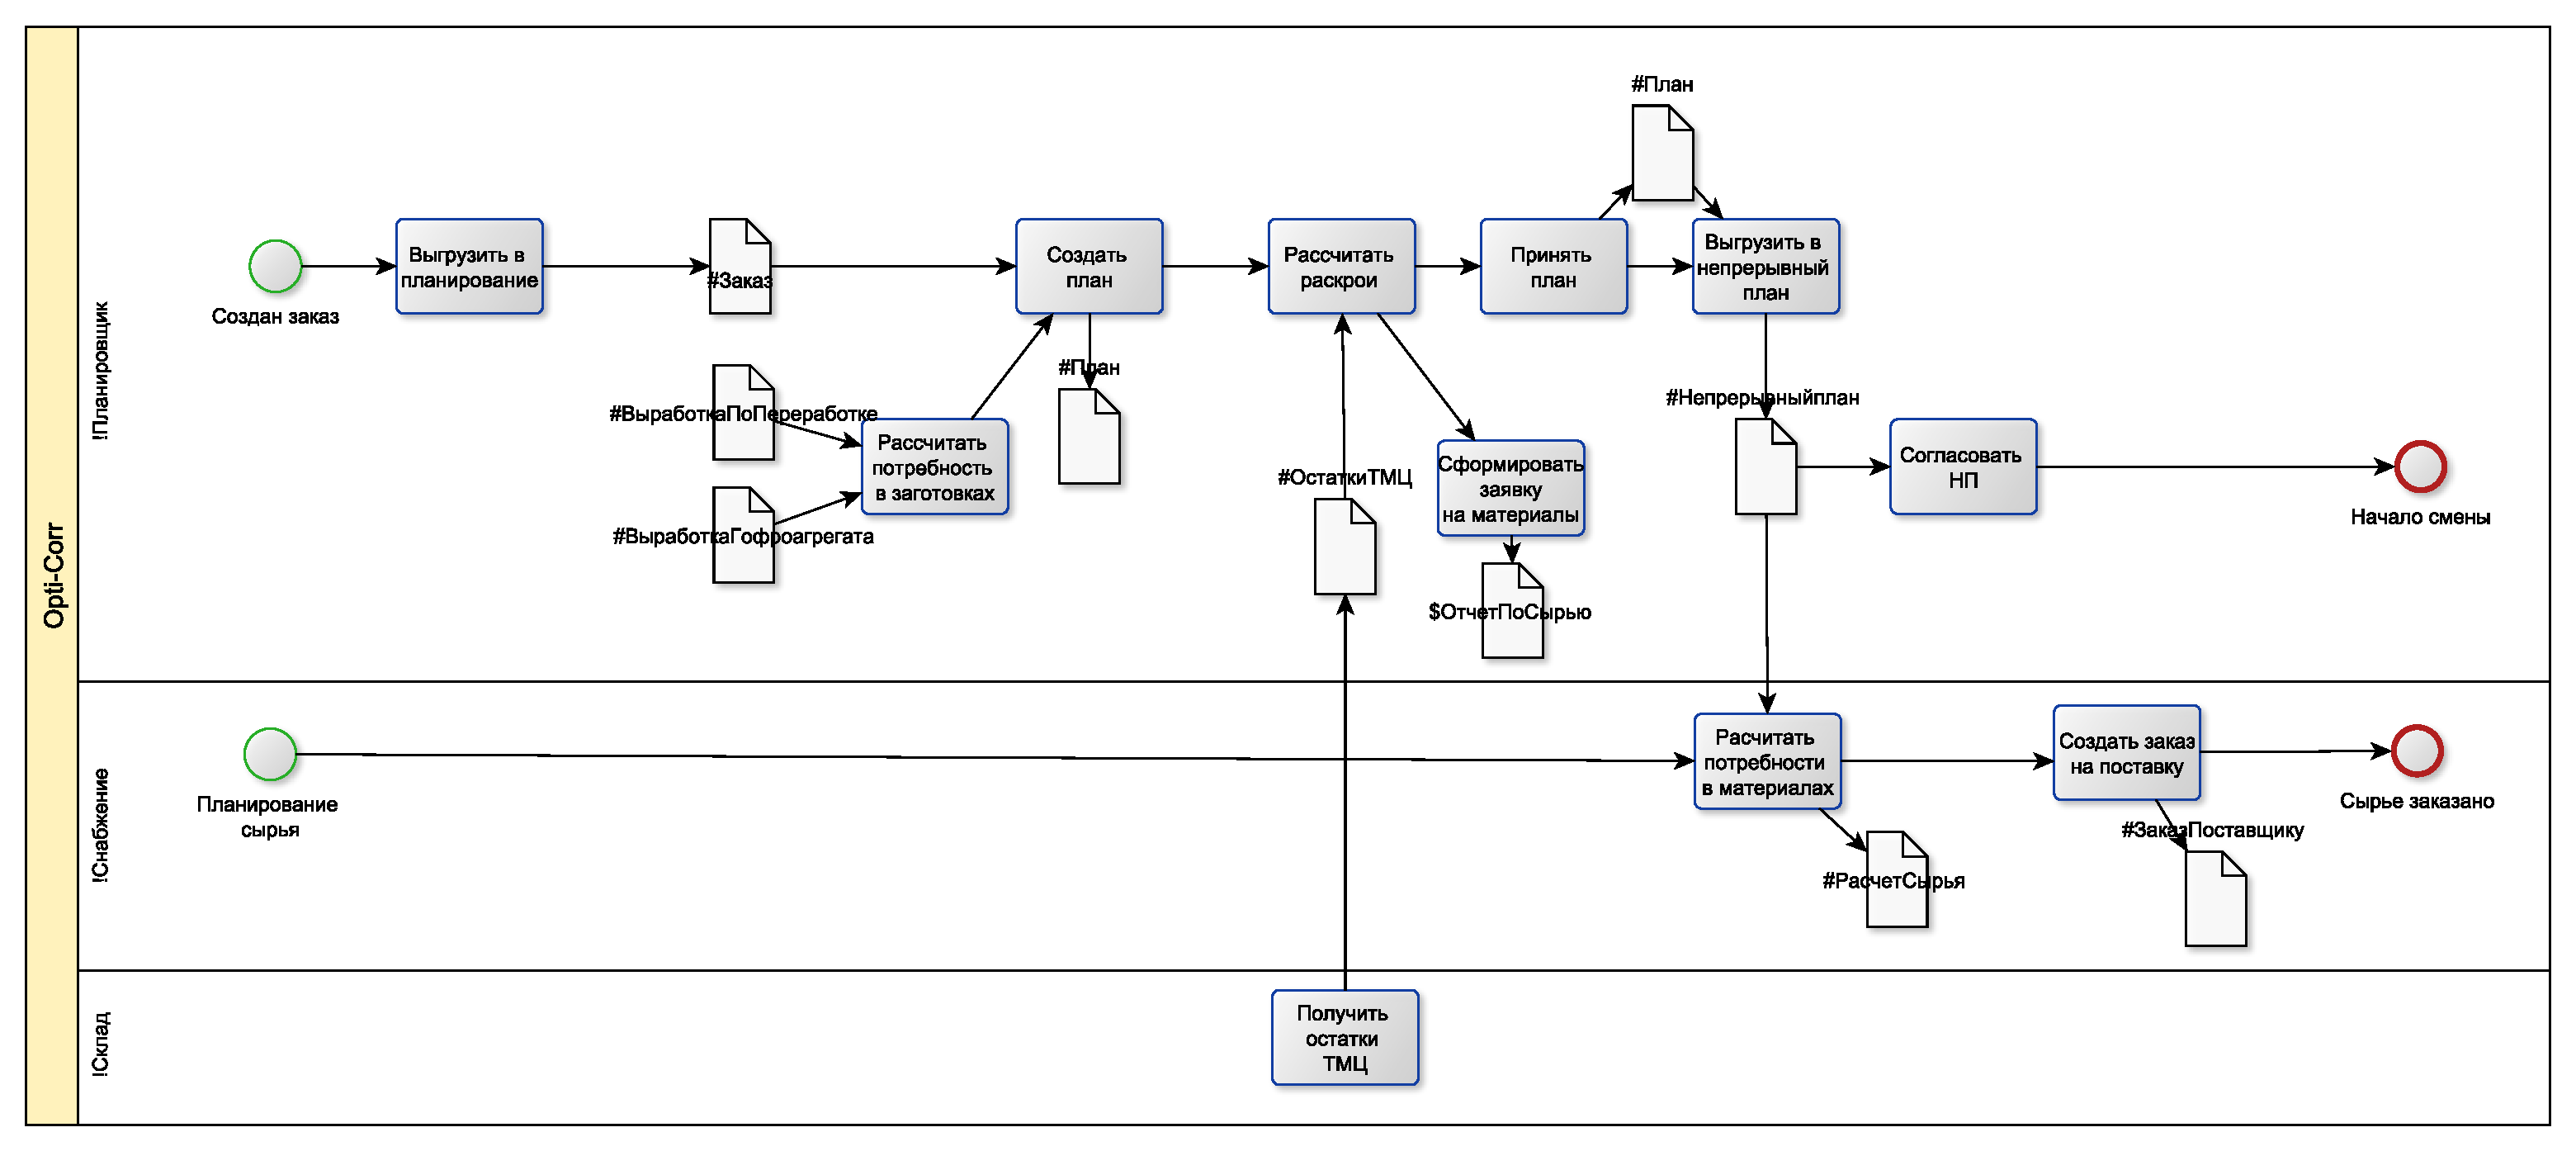
\includegraphics[angle=90, height=0.8\textheight, keepaspectratio]{Pics/3_Plan.pdf}
\end{center}
  \caption{Процессы ''Предварительное планирование'', ''Оперативное планирование''}
  \label{pic:Schema_3}
\end{figure}
\clearpage


Из отдела продаж заказы с одобренным статусом появляются в СИСТЕМЕ у планировщика.

Планировщик выполняет оперативное планирование работы гофроагрегата и линий переработки. По факту планирования работы гофроагрегата, Планировщик в СИСТЕМЕ формирует потребности по материалам, создает документ ''Заказ поставщику''. 
В результате Планировщик формирует оперативный план работы по гофроагрегату и линиям переработки.
План производства доступен на производстве для выполнения.



% По регламенту СИСТЕМА выгружает все складские документы в систему 1С:УНФ.
% %
% %\newpage
% %%
\subsection{Процессы ''Управление производством''}
%
\begin{figure}
\begin{center}
  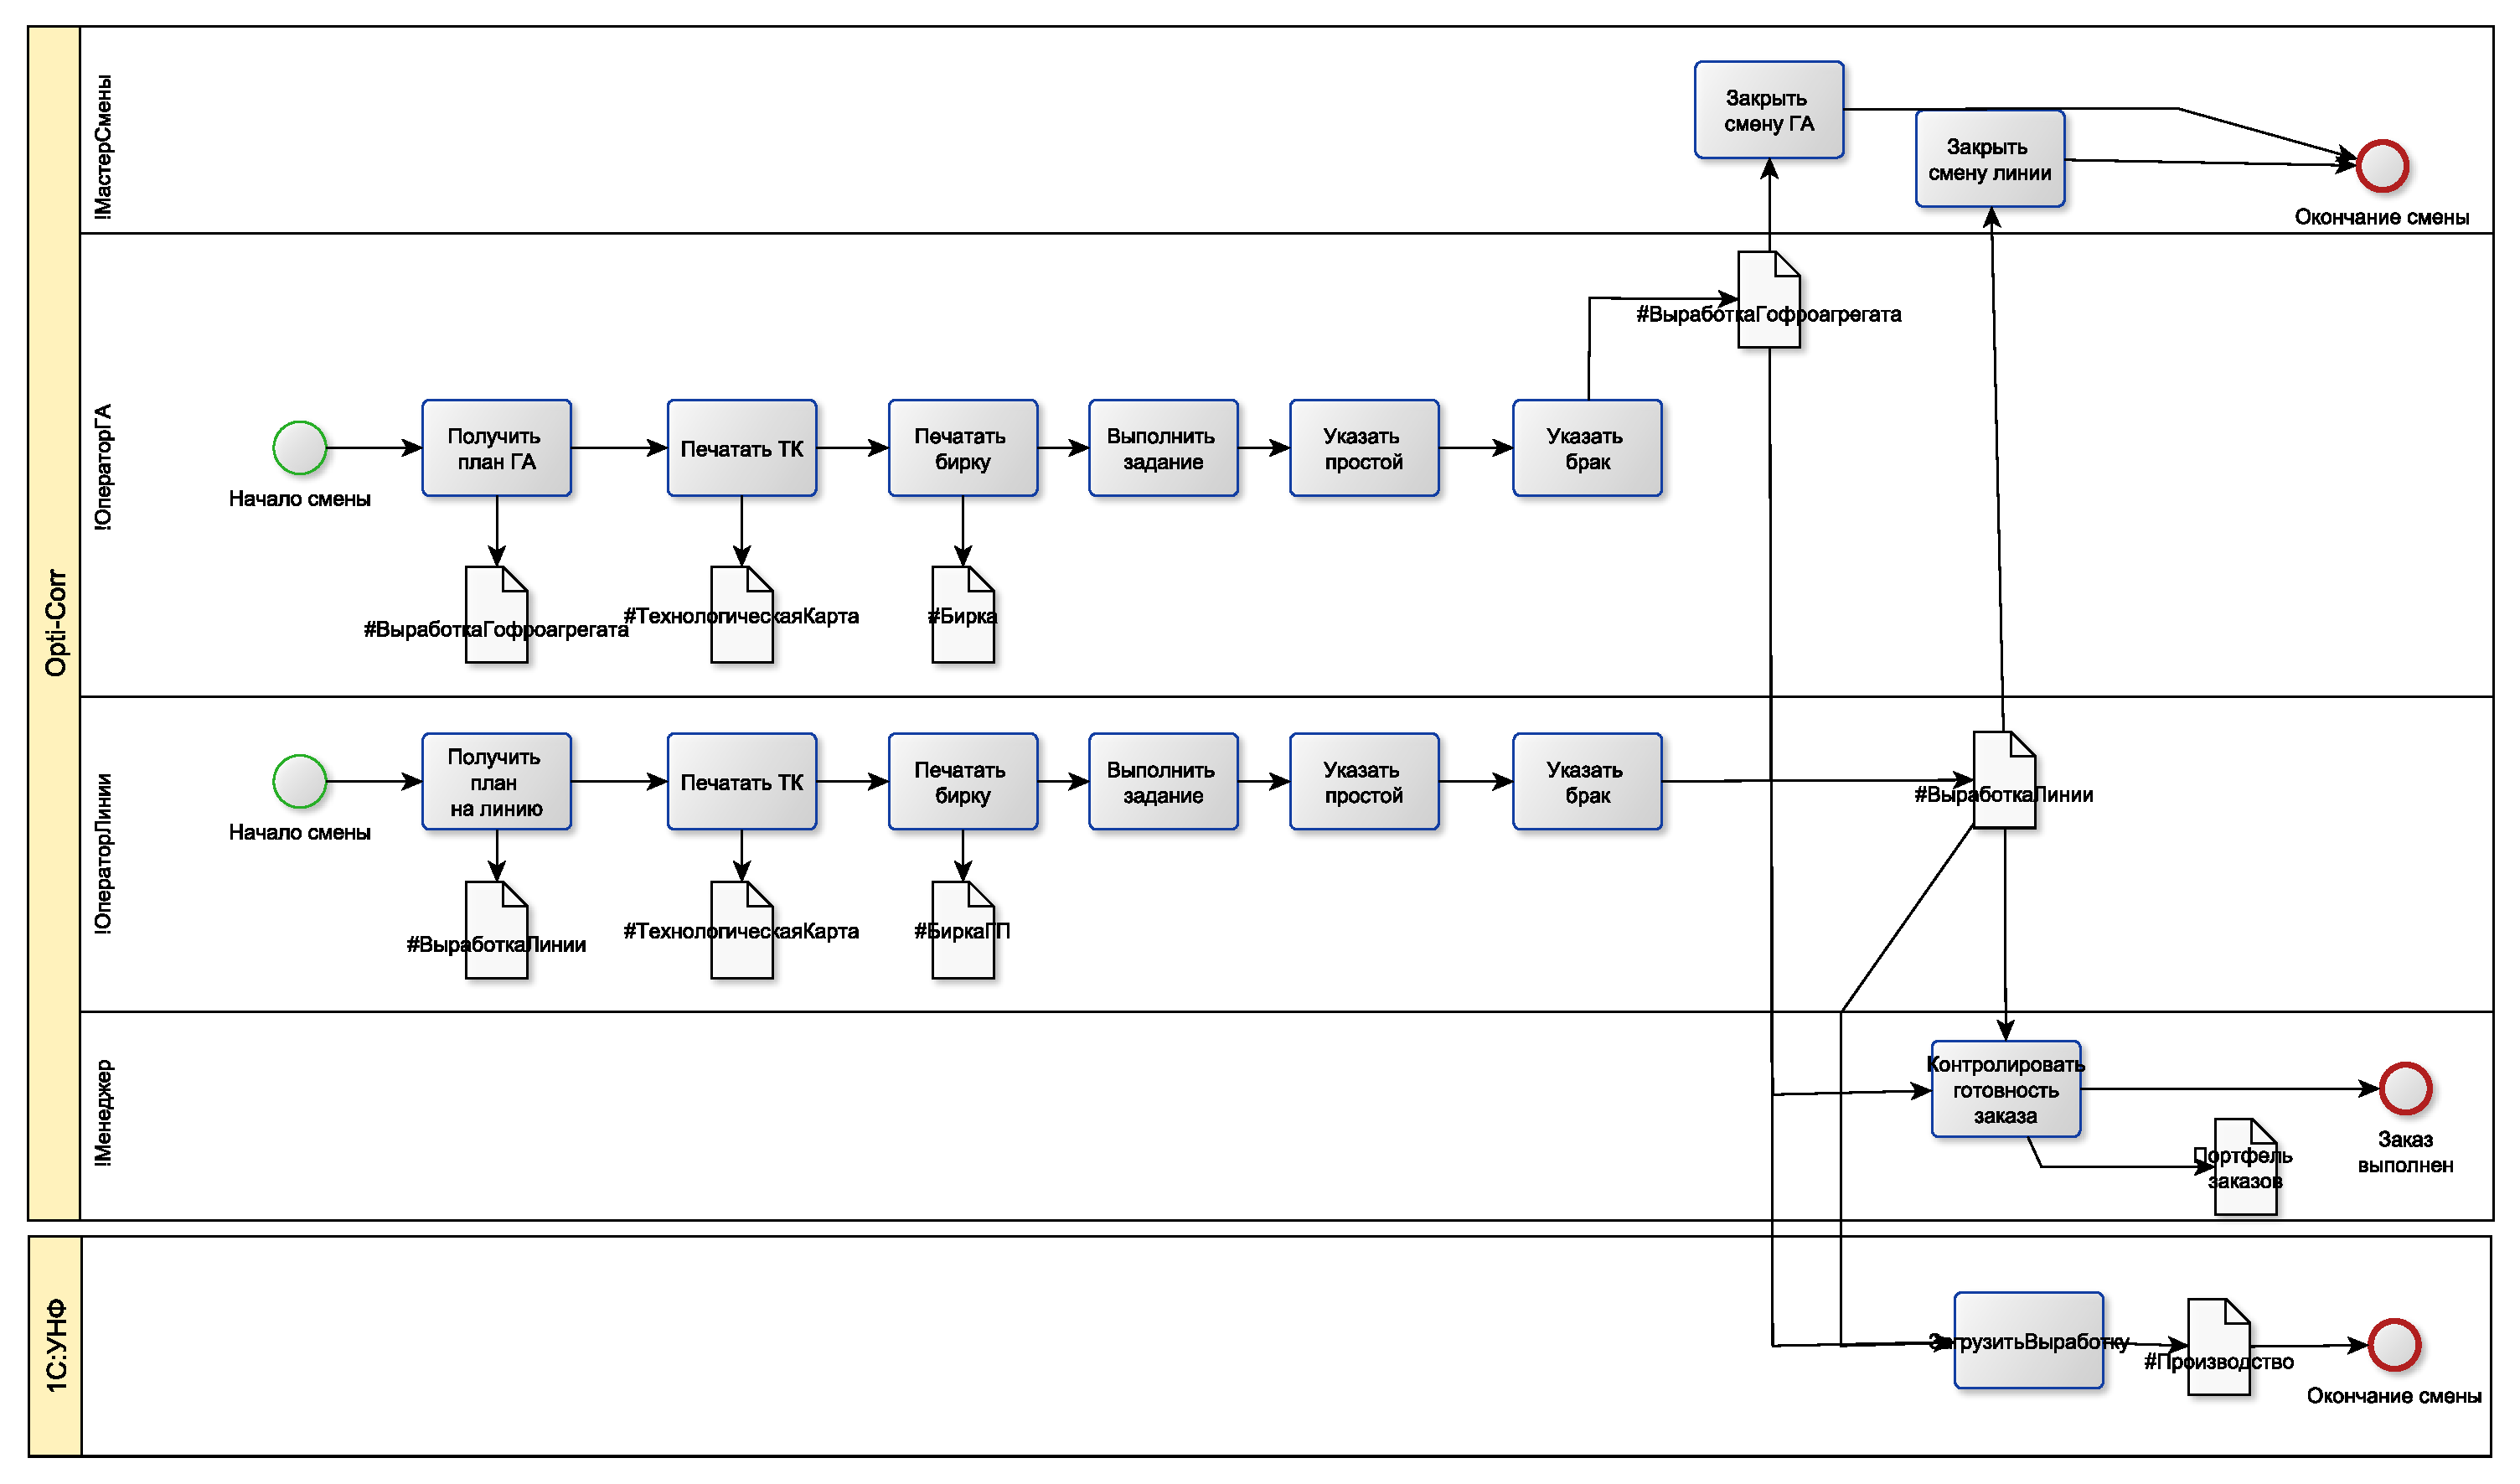
\includegraphics[angle=90, height=0.9\textheight, keepaspectratio]{Pics/4_Output.pdf}
\end{center}
  \caption{Процессы ''Управление производством''}
  \label{pic:Schema_4}
\end{figure}
% \clearpage




 Машинист гофроагрегата получает оперативный план производства на своем рабочем месте в СИСТЕМЕ. Машинист гофроагрегата должен в СИСТЕМЕ зафиксировать выработку по гофроагрегату (в документе ''Выработка гофроагрегата''), в т.ч. брак в работе гофроагрегата, простои и неисправности.

Рабочее место машиниста будет подключено к гофроагрегату Hsien Hsu. По команде машиниста раскрои будут выгружаться автоматически в память гофроагрегата.
После выполнения раскроя данные по выработке будут загружены в рабочее место в СИСТЕМУ.

Машинист на технологической линии получает оперативный план производства линии на своем рабочем месте в СИСТЕМЕ. Машинист технологической линии фиксирует факт выработки по заказу, отклонения, в т.ч. брак при работе линии, простои и неисправности (см. рис. \ref{pic:Schema_4}).

% Документы по выработке ''Выработка гофроагрегата'', ''Выработка по переработке'' при автоматическом обмене СИСТЕМА выгрузит в документы ''Отчет производства'' в систему 1С:УНФ.



\subsection{Процессы ''Планирование отгрузки'', ''Управление качеством'', ''Управление продажами''}
%
\begin{figure}
\begin{center}
  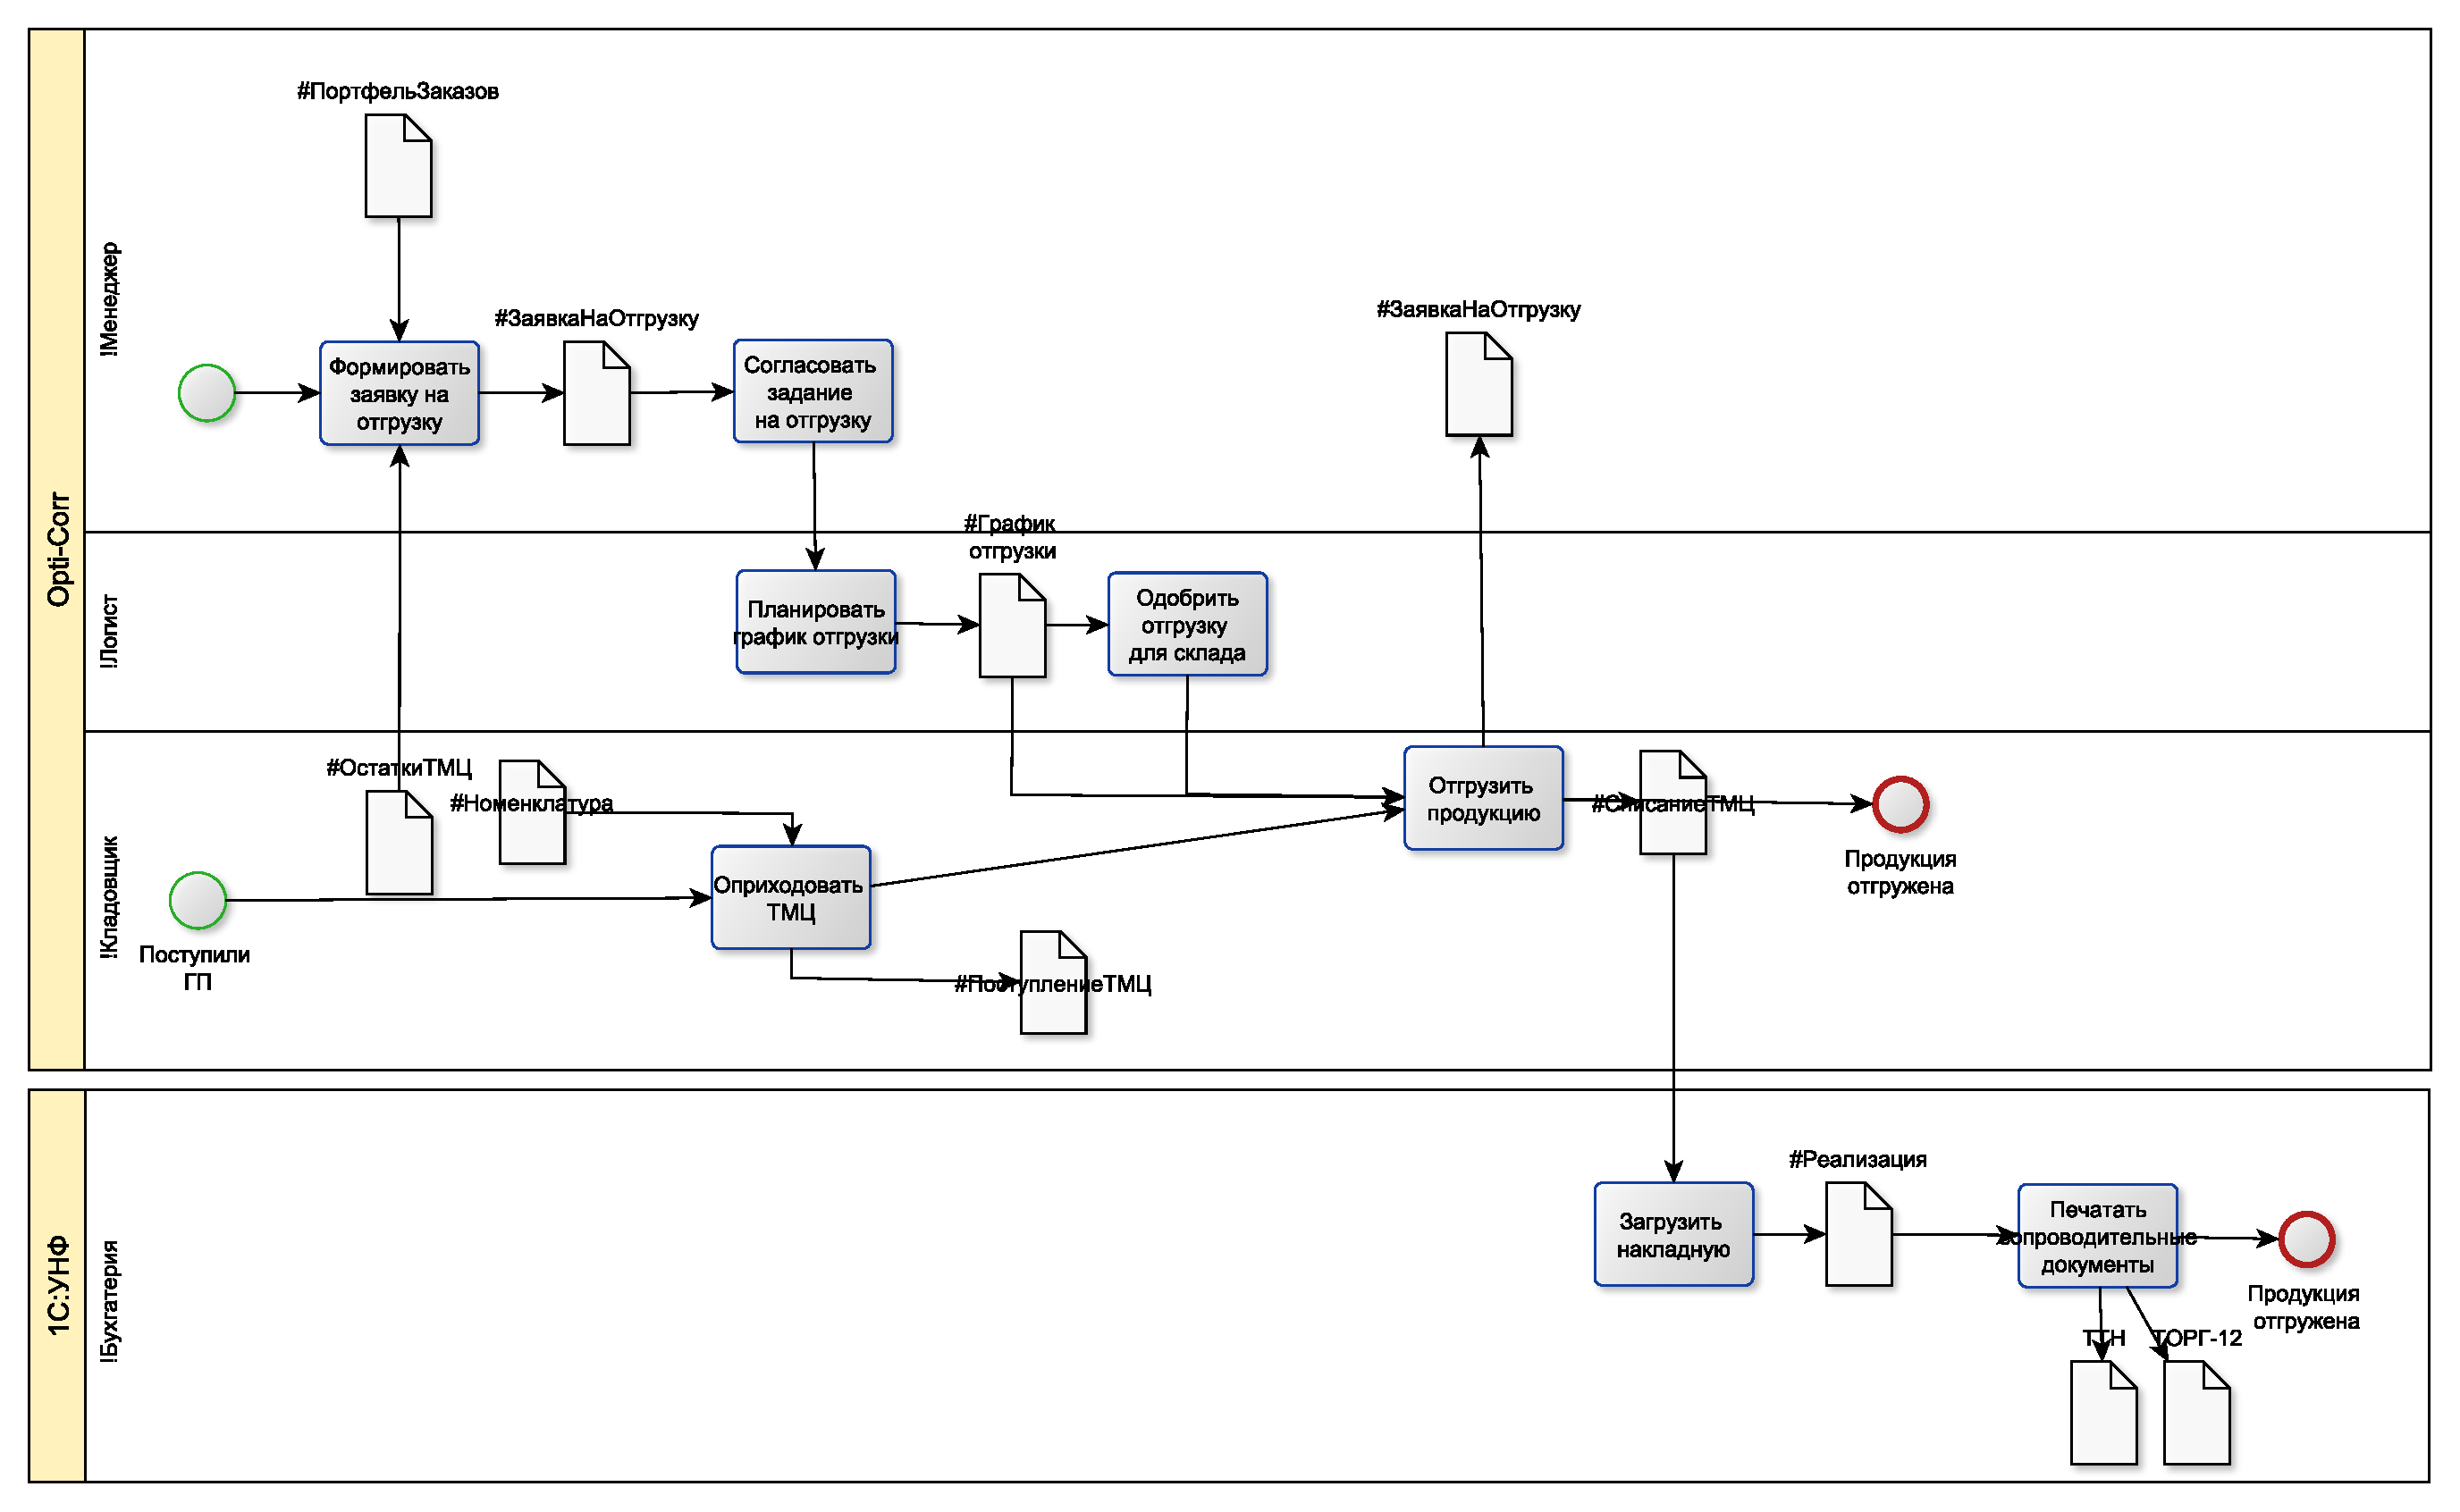
\includegraphics[angle=90, height=0.9\textheight, keepaspectratio]{Pics/5_Shipment.pdf}
\end{center}
  \caption{Процессы ''Планирование отгрузки'', ''Управление качеством'', ''Управление продажами''}
  \label{pic:Schema_5}
\end{figure}
% \clearpage



Цена продукции по умолчанию будет указана в справочнике ''Номенклатура'' менеджером.


По факту изготовления готовой продукции менеджер будет контролировать в СИСТЕМЕ состояние заказа, его готовность и местоположение.
При готовности заказа менеджер будет создавать в СИСТЕМЕ документ ''Заявка на отгрузку'' либо вручную, либо на основании заявки покупателя.
Логист отдела продаж в СИСТЕМЕ указывает в документах ''Заявка на отгрузку'' транспорт, который будет подан под погрузку. Логист планирует транспорт под погрузку.

Логист планирует размещение груза в транспортном средстве в СИСТЕМЕ через оптимизатор погрузки.

Заявка на отгрузку будет автоматически или по запросу выгружена из СИСТЕМЫ в систему 1С:УНФ в документ "ЗаявкаНаОтгрузку".

Отгрузка готовой продукции будет выполняться в СИСТЕМЕ кладовщиком на основании документа ''ЗаявкаНаОтгрузку'' (см. рис. \ref{pic:Schema_5}).

% Кладовщик на производстве будет видеть в системе 1С:УНФ все распоряжения на отгрузку (Заявка на отгрузку).
% При поступлении транспорта кладовщик создает на основании документа ''Распоряжение на отгрузку'' документ ''Реализация ТМЦ''. По факту отгрузки кладовщик корректирует при необходимости факт отгрузки в документе ''Реализация ТМЦ''. 

Кладовщик печатает сопроводительные документы в системе 1С:УНФ: ТН, ТТН.
Бухгалтер печатает сопроводительные документы в системе 1С:УНФ: счет-фактура, расходная накладная.

% Документы ''Реализация ТМЦ''  при автоматическом обмене СИСТЕМА выгрузит в документы ''Реализация'' в систему 1С:УНФ.


% %
% %
\subsection{Процессы ''Поступление материалов'', ''Списание материалов в производство''}
%
\begin{figure}
\begin{center}
  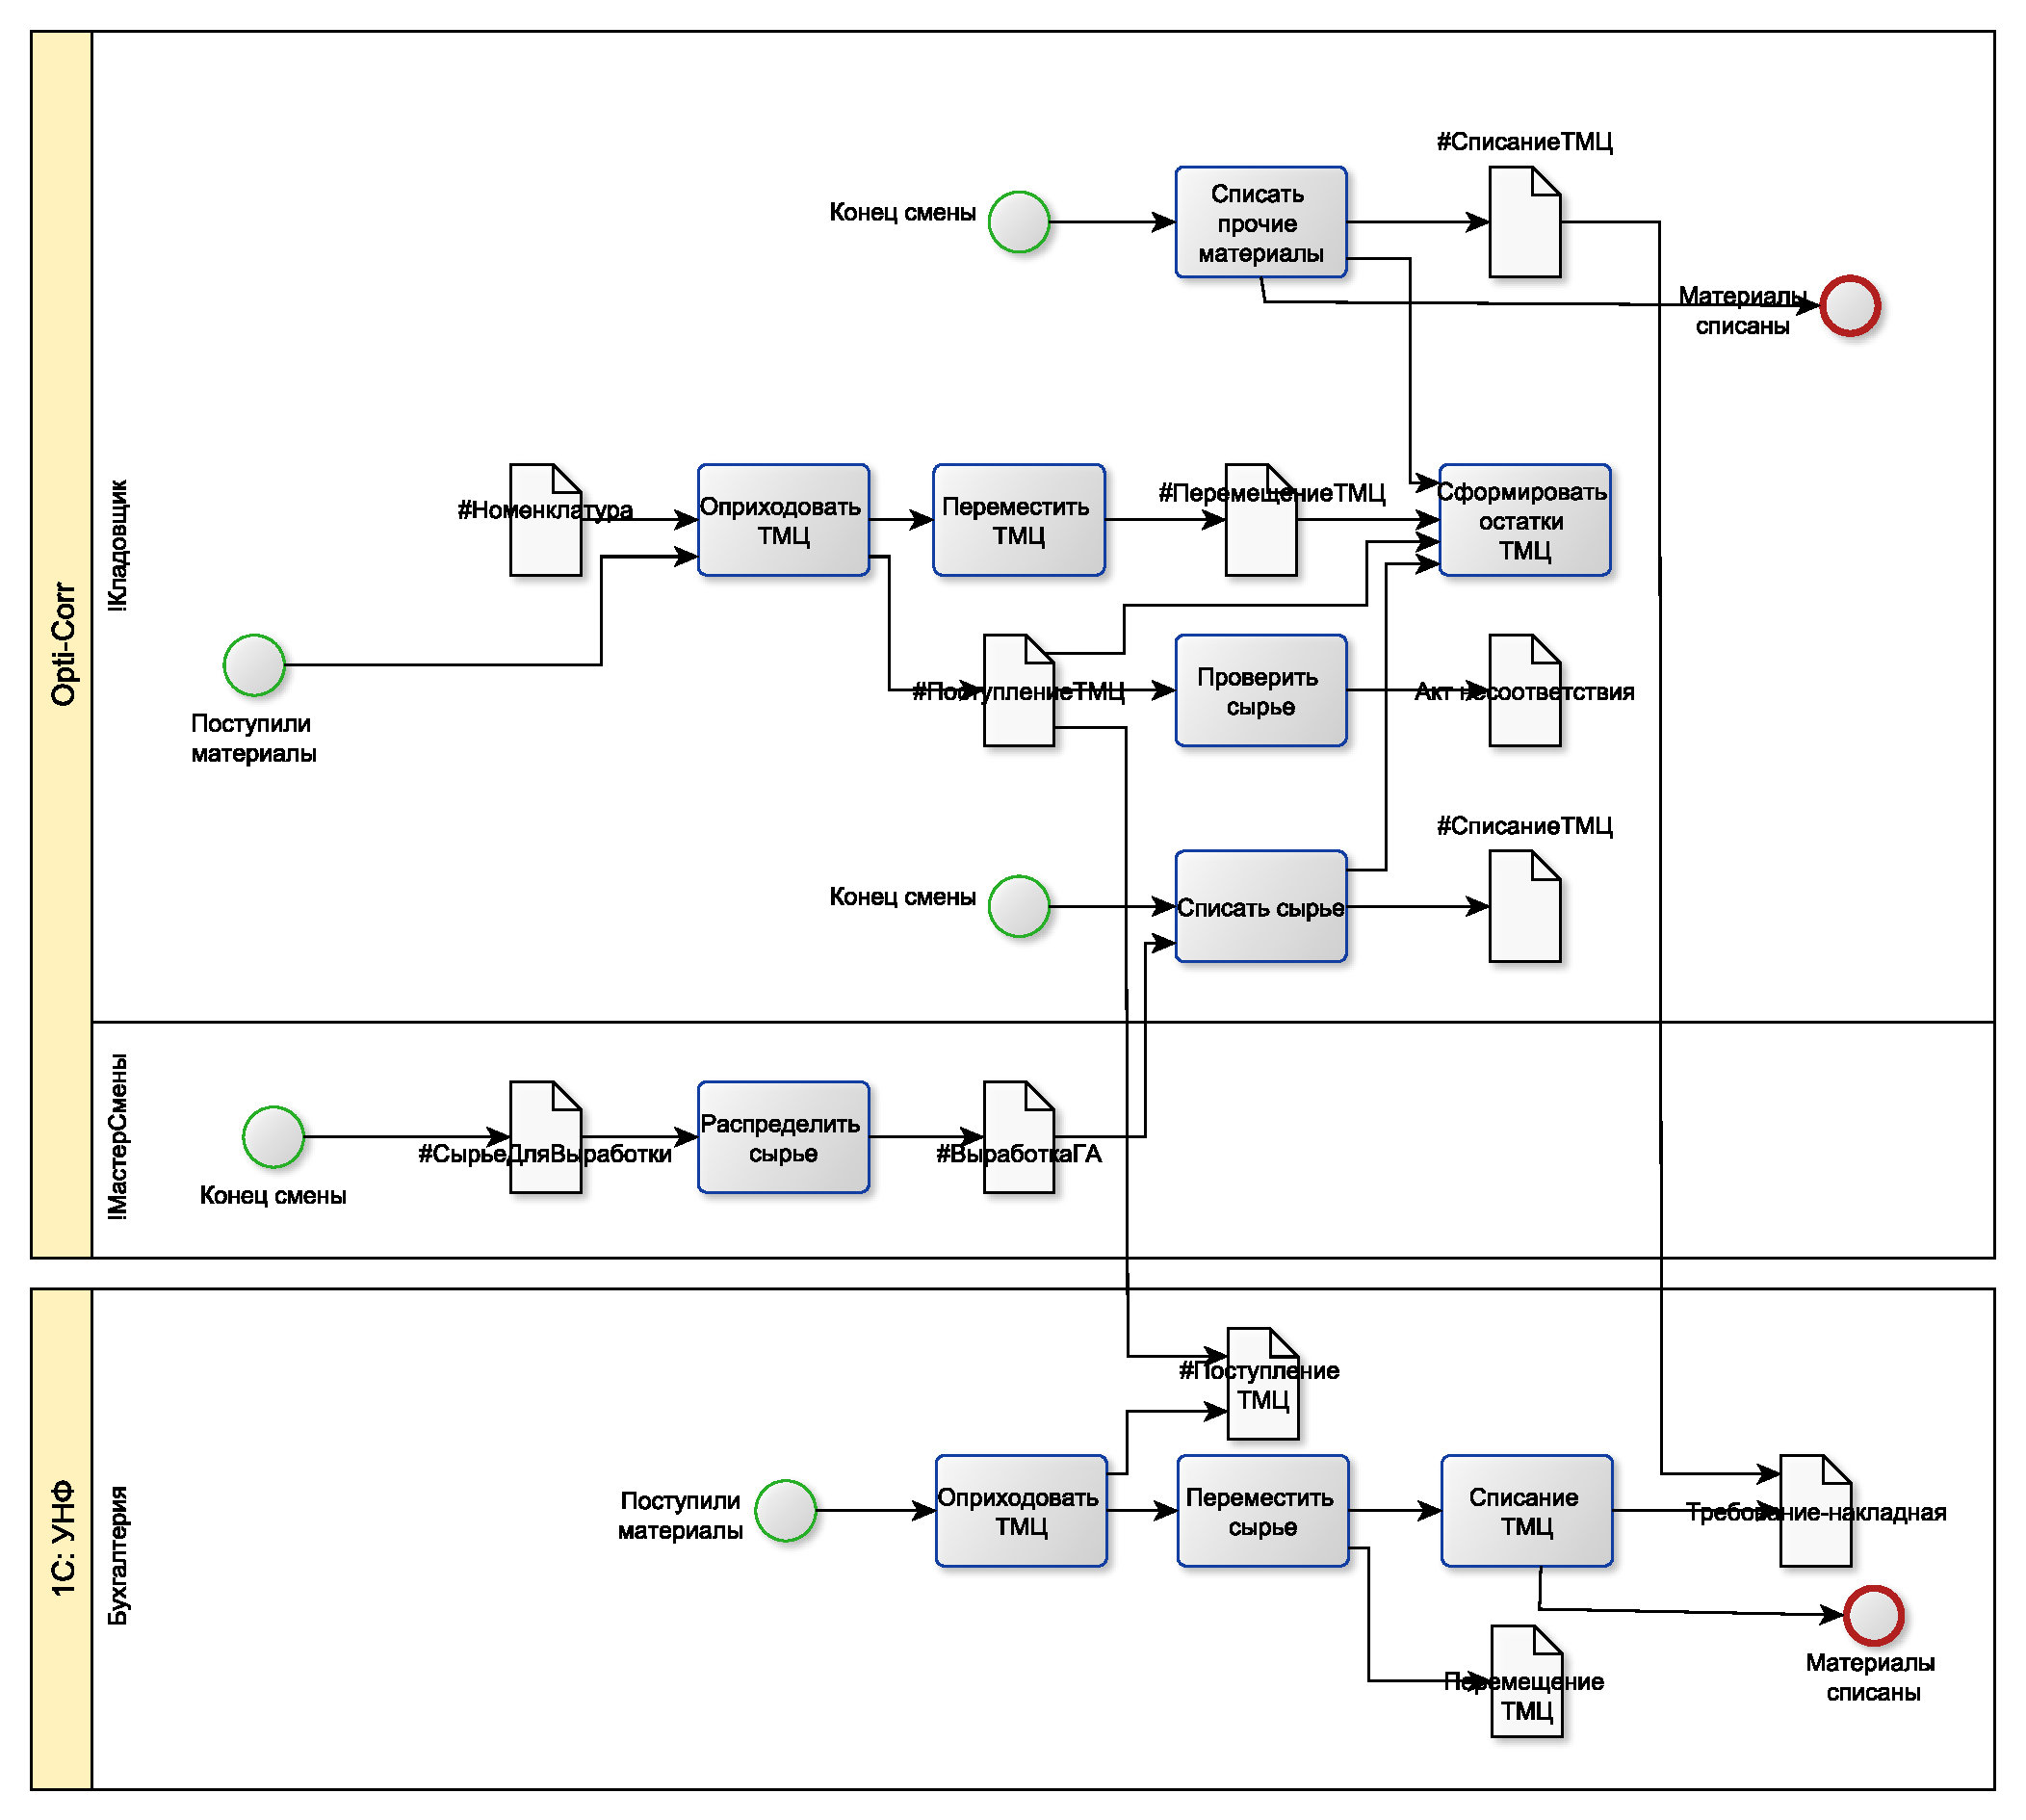
\includegraphics[angle=90, height=0.8\textheight, keepaspectratio]{Pics/6_Warehouse.pdf}
\end{center}
  \caption{Процессы ''Поступление материалов'', ''Списание материалов в производство''}
  \label{pic:Schema_6}
\end{figure}
% \clearpage

% Учет материалов остается в системе 1С:УНФ как есть.

Материалы (заготовки) будет оприходовать мастер производства в системе Опти-Софт документом ''Поступление ТМЦ''. Рулоны бумаги и картона оприходует кладовщик 
в системе Опти-Софт документом ''Поступление ТМЦ''.

При необходимости перемещения рулонов на гофроагрегат кладовщик создает документ ''Перемещение ТМЦ'' в системе Опти-Софт.

% Кладовщик на производстве в СИСТЕМЕ оприходует поступающие материалы и заготовки в СИСТЕМЕ в документе "Поступление ТМЦ". 
% Мастер на производстве фиксирует перемещение ТМЦ документом "Перемещение ТМЦ".

% Операторы на раскатах фиксируют сырье, использованное при производстве гофрокартона, в документе "Сырье для выработки".
% Кладовщик выполняет списание в производство  в СИСТЕМЕ документом ''Списание ТМЦ'' на основании документа "Сырье для выработки".

Документы автоматически выгружаются в систему 1С:УНФ по регламенту (см. рис. \ref{pic:Schema_6}).

%
%
%
%
%
%%
%%\newpage
%%
%%\subsection{Процессы 'Управление и диспетчеризация производства', 'Списание бумаги и картона', 'Управление качеством', 'Учет готовой продукции', 'Планирование отгрузки', 'Отгрузка готовой продукции'}
%%
%%\begin{figure}
%%\begin{center}
%%  \includegraphics[height=0.94\textheight, keepaspectratio]{Pics/Schema_3.jpg}
%%\end{center}
%% % \caption{Процессы 'Управление и диспетчеризация производства', 'Списание бумаги и картона', 'Управление качеством', 'Учет готовой продукции', 'Планирование отгрузки', 'Отгрузка готовой продукции'}
%%  \label{pic:Schema_3}
%%\end{figure}
%%\clearpage
%